\documentclass[aspectratio=169]{beamer}

\usepackage{calc}
\usepackage{graphicx}
\usepackage{siunitx}
\usepackage{xcolor}

\graphicspath{{./images}}
\setbeamertemplate{navigation symbols}{}

\author{Chris Doble}
\date{}
\subtitle{Building a GPS receiver from scratch}
\title{Part 4: Sampling}
\usetheme{Madrid}

% Show the topics frame at the start of each section
\AtBeginSection[]
{
  \begin{frame}
    \frametitle{Topics}
    \tableofcontents[currentsection]
  \end{frame}
}

% Show the topics frame at the start of each subsection
\AtBeginSubsection[]
{
  \begin{frame}
    \frametitle{Topics}
    \tableofcontents[currentsection, currentsubsection]
  \end{frame}
}

\begin{document}

\frame{\titlepage}

\begin{frame}
    \frametitle{Topics}

    \tableofcontents
\end{frame}

\section{Hardware}

\begin{frame}
    \frametitle{Hardware}

    \begin{itemize}
        \item Software defined radio (SDR) dongle
    \end{itemize}

    \leavevmode \\

    \centering
    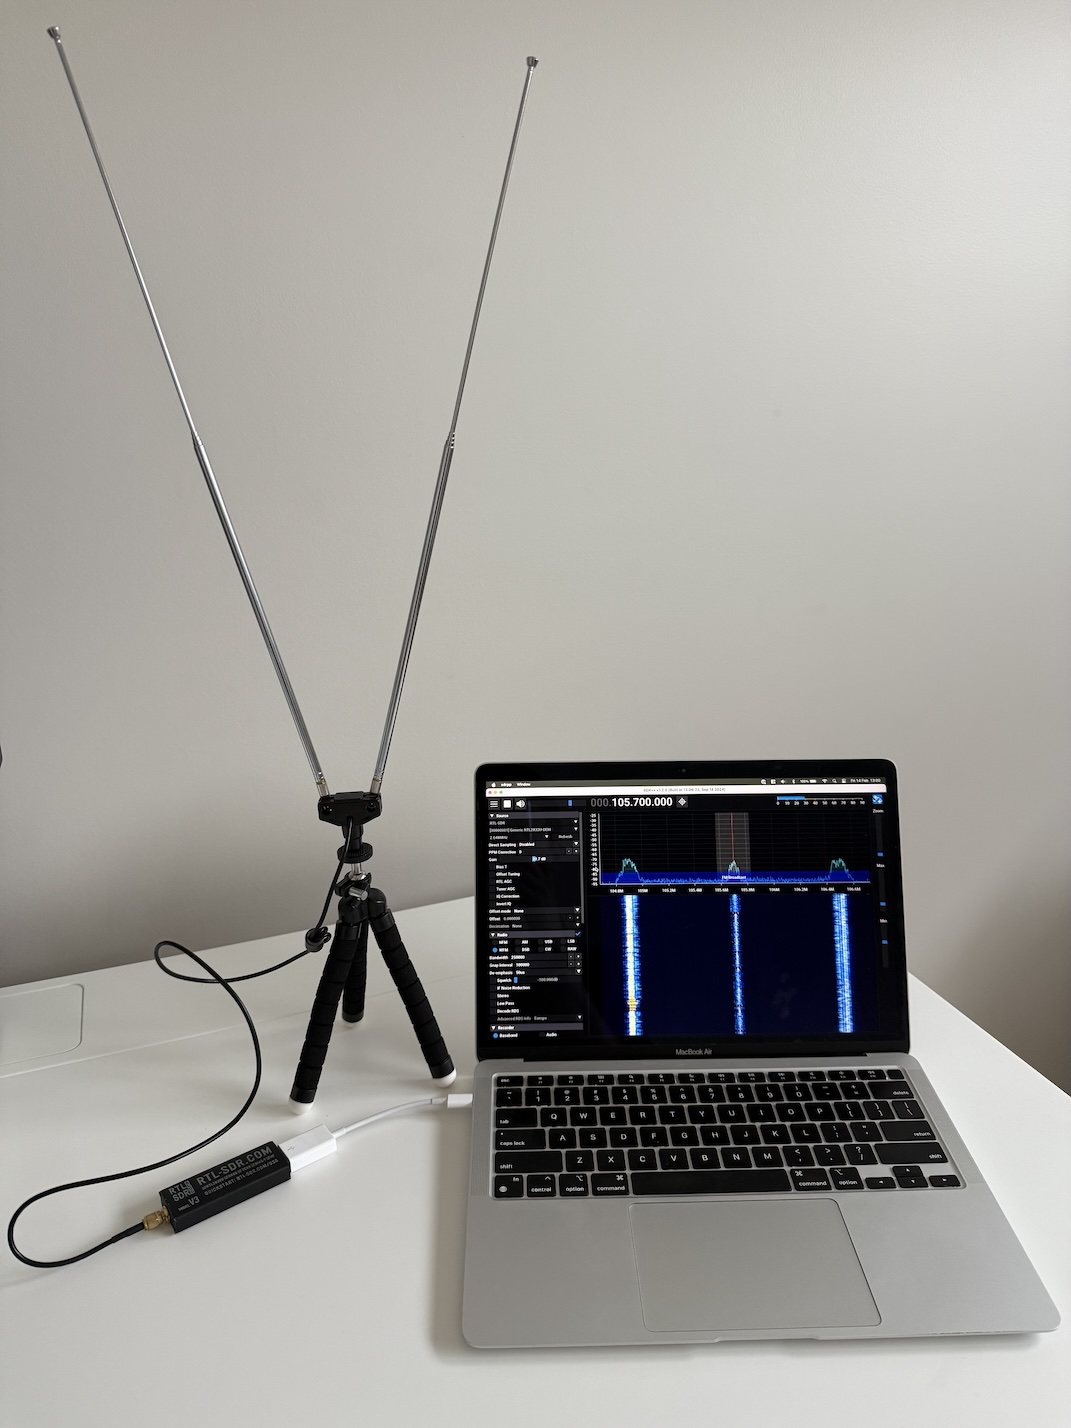
\includegraphics[width=\textwidth * 4 / 15]{1 hardware.jpg}
\end{frame}

\begin{frame}
    \frametitle{Hardware}

    \centering
    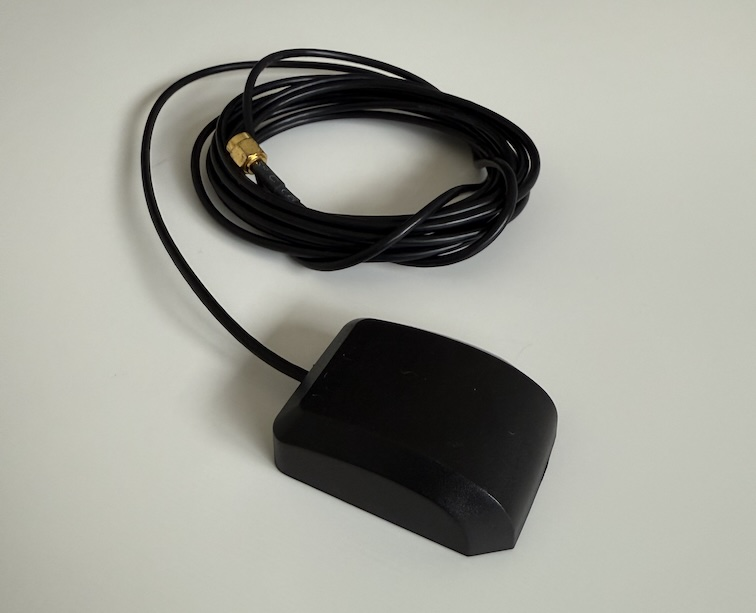
\includegraphics[width=\textwidth / 2]{2 GPS antenna.jpg}
\end{frame}

\section{Parameters}

\subsection{Centre frequency}

\begin{frame}
    \frametitle{Centre frequency}

    \Large
    \[f = \qty{1575.42}{MHz}\]
\end{frame}

\subsection{Bandwidth}

\begin{frame}
    \frametitle{The power spectrum of BPSK}

    \centering
    \only<1>{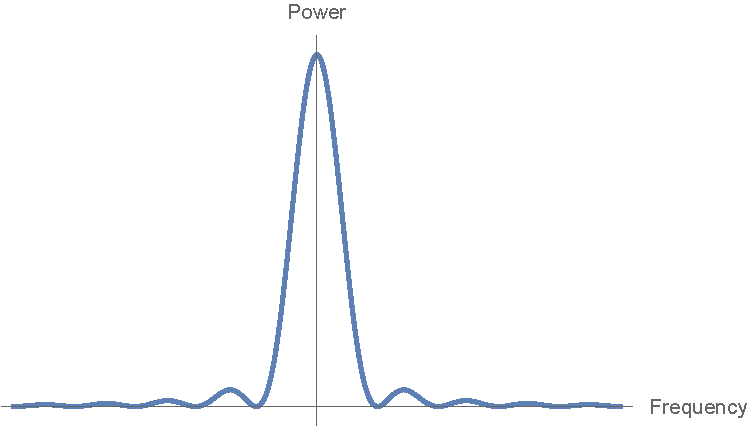
\includegraphics{3 BPSK PSD.pdf}}%
    \only<2>{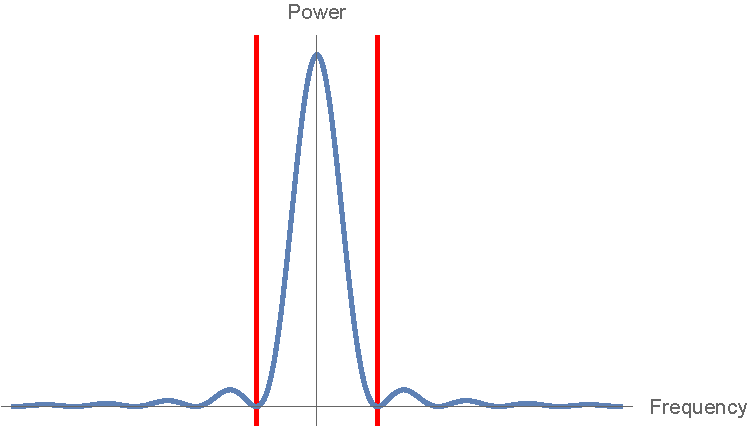
\includegraphics{4 BPSK PSD main lobe.pdf}}
\end{frame}

\begin{frame}
    \frametitle{Bandwidth}

    \Large
    \[B = \qty{2.046}{MHz}\]
\end{frame}

\subsection{Sampling rate}

\begin{frame}
    \frametitle{Sampling rate}

    \Large
    \[f_{L1} = \qty{1575.42}{Mhz} \approx \qty{1.6}{GHz}\]
\end{frame}

\begin{frame}
    \frametitle{The Nyquist-Shannon sampling theorem}

    \centering
    \Large
    If the maximum frequency contained within a signal is $f_\text{max}$,\\then the signal can be determined from its samples\\if the sampling rate is greater than $2 f_\text{max}$.
\end{frame}

\begin{frame}
    \frametitle{Sampling rate}

    \Large
    \begin{align*}
    f_\text{max} &= f + \frac{B}{2} \\
    \onslide<2->{&= \qty{1575.42}{MHz} + \frac{\qty{2.046}{MHz}}{2} \\}
    \onslide<3->{&= \qty{1576.443}{MHz} \\}
    \onslide<3->{& \approx \qty{1.6}{GHz} \\}
    \onslide<4->{f_s &= 2 f_\text{max} \\}
    \onslide<4->{& \approx \qty{3.2}{GHz}}
    \end{align*}
\end{frame}

\begin{frame}
    \frametitle{Sampling rate}

    \centering
    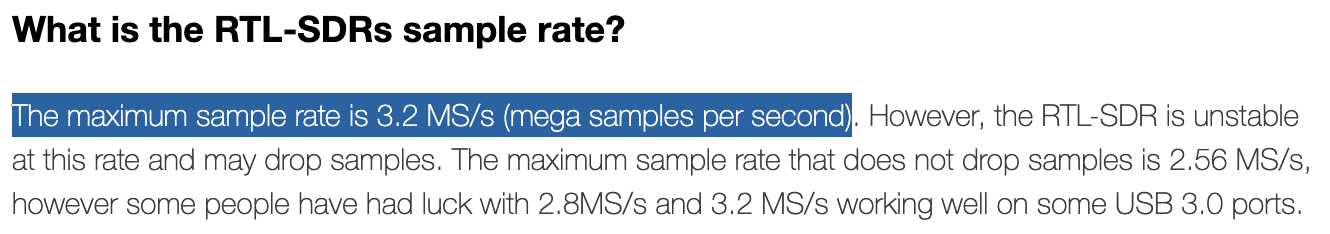
\includegraphics[width=\textwidth]{5 RTL-SDR maximum sampling rate.png}
    \texttt{\tiny{https://www.rtl-sdr.com/about-rtl-sdr/}}
\end{frame}

\begin{frame}
    \frametitle{Sampling rate}

    {\Large \[f_s = \qty{2.046}{MHz}\]}

    \leavevmode \\

    \begin{itemize}
        \item<2-> Large enough that aliases don't overlap
        
        \item<3-> $1 / 770$ of the L1 frequency $\Rightarrow$ alias at $\qty{0}{Hz}$
        
        \item<4-> $f_\text{max} = \qty{1.023}{MHz} \Rightarrow f_\text{Nyquist} = \qty{2.046}{MHz} \Rightarrow$ within SDR dongle's capabilities
    \end{itemize}
\end{frame}

\section{I/Q samples}

\subsection{Definition}

\begin{frame}
    \frametitle{The definition of I/Q samples}

    \Large
    \only<1-3>{
        \only<1-2>{\[f(t) = A(t) \cos(2 \pi f t + \phi(t))\]}
        \only<3->{\[f(t) = A(t) \, \textcolor{red}{\cos(2 \pi f t + \phi(t))}\]}
        \onslide<2->{\[\cos(\alpha + \beta) = \cos(\alpha) \cos(\beta) - \sin(\alpha) \sin(\beta)\]}
    }
    \only<4-6>{
        \only<4-5>{\[f(t) = A(t) [\cos(2 \pi f t) \cos(\phi(t)) \, \textcolor{black}{- \sin(2 \pi f t)} \sin(\phi(t))]\]}
        \only<6->{\[f(t) = A(t) [\cos(2 \pi f t) \cos(\phi(t)) \, \textcolor{red}{- \sin(2 \pi f t)} \sin(\phi(t))]\]}
        \onslide<5->{\[-\sin(\theta) = \cos(\theta + \pi / 2)\]}
    }
    \only<7->{
        \begin{align*}
            f(t) &= A(t) [\cos(2 \pi f t) \cos(\phi(t)) + \cos(2 \pi f t + \pi / 2) \sin(\phi(t))] \\
            \onslide<8->{&= A(t) \cos(\phi(t)) \cos(2 \pi f t) + A(t) \sin(\phi(t)) \cos(2 \pi f t + \pi / 2) \\}
            \onslide<9->{&= I(t) \cos(2 \pi f t) + Q(t) \cos(2 \pi f t + \pi / 2)}
        \end{align*}

        \onslide<9->{where $I(t) = A(t) \cos(\phi(t))$ and $Q(t) = A(t) \sin(\phi(t))$.}
    }
\end{frame}

\begin{frame}
    \frametitle{Determining a signal's phase}

    \Large
    \begin{align*}
        Q / I &= \onslide<2->{\frac{A(t) \sin(\phi(t))}{A(t) \cos(\phi(t))}} \\
        \onslide<3->{&= \tan(\phi(t))} \\
        \onslide<4->{\phi(t) &= \arctan(Q / I)}
    \end{align*}
\end{frame}

\subsection{Different frequencies}

\begin{frame}
    \frametitle{Sampling a signal of a different frequency}

    \Large
    \begin{align*}
        \onslide<2->{f_1 & \\}
        \onslide<3->{f_2 & = f_1 + \Delta f} \\
        \onslide<4->{f(t) &= A \cos (2 \pi f_2 t) \\}
        \onslide<5->{&= A \cos (2 \pi (f_1 + \Delta f) t) \\}
        \onslide<5->{&= A \cos (2 \pi f_1 t + 2 \pi \Delta f t) \\}
        \onslide<6->{&= A \cos (2 \pi f_1 t + \phi(t))}
    \end{align*}

    \onslide<6->{where $\phi(t) = 2 \pi \Delta f t$.}
\end{frame}

\subsection{Complex values}

\begin{frame}
    \frametitle{Complex I/Q samples}

    \begin{itemize}
        \item<1-> $I + j Q$
        
        \item<2-> Bandpass sampling
        
        \begin{itemize}
            \item<3-> Real-valued samples $\Rightarrow$ carrier wave replaced with a real-valued constant
        
            \item<4-> Complex-valued samples $\Rightarrow$ carrier wave replaced with a complex-valued constant
            
            \item<5-> Using Euler's formula $z = A e^{j \phi}$ where $A$ is the carrier wave's amplitude and $\phi$ is its phase
        \end{itemize}

        \onslide<6->{
            \begin{align*}
                \onslide<6->{\hat{D}_i(t) \hat{PRN}_i(t) &= \pm 1 \\}
                \onslide<7->{z \hat{D}_i(t) \hat{PRN}_i(t) &= z (\pm 1) \\}
                \onslide<7->{&= A e^{j \phi} (\pm 1) \\}
                \onslide<7->{&= \pm A e^{j \phi}}
            \end{align*}
        }
    \end{itemize}
\end{frame}

\begin{frame}
    \frametitle{Recap}

    \begin{itemize}
        \item<2-> Hardware
        
        \begin{itemize}
            \item GPS antenna
            
            \item SDR dongle
        \end{itemize}

        \item<3-> Parameters
        
        \begin{itemize}
            \item Central frequency $f = \qty{1575.42}{MHz}$
            
            \item Bandwidth $B = \qty{2.046}{MHz}$
            
            \item Sampling rate $f_s = \qty{2.046}{MHz}$
        \end{itemize}

        \item<4-> I/Q samples
        
        \begin{itemize}
            \item<5-> Pairs of numbers that describe the signal

            \item<6-> Often expressed as a single complex number
            
            \item<7-> If the signal has a different frequency, the I/Q samples will continually rotate
        \end{itemize}
    \end{itemize}
\end{frame}

\end{document}